\chapter{Techniques and algorithms}
\label{chap:ch2}

In his 1950 paper, "Programming a Computer for Playing Chess" \cite{shannon1950xxii}, Claude E. Shannon describes how a chess engine might be implemented. Although not clearly stated, from his work we can deduce the three main parts a machine would need to do to be able to play chess, which are still valid and used in modern engines:
\begin{itemize}
    \item Generating the legal moves of a position
    \item Searching for legally reachable positions from a position
    \item Evaluating the positions
\end{itemize}

\section{Move generation}
\label{sec:ch2sec1}

\subsection{Legality}
\label{subsec:ch2sec1subsec1}

Regarding legality of the moves, move generation can be pseudo-legal or legal. In pseudo-legal move generation, the moves generated follow the normal rules of each piece's movement, but they are not checked to see if the king is left or moved into check. In legal move generation only legal moves are generated, checking beforehand if the king would be left in an illegal position. Pins, along with en passant moves, are particularly difficult to check. That is why the first approach is generally used: generating the pseudo-legal moves first, checking each move to see if it leaves the board in a valid state (the king of the side that moved is not in check), and removing the invalid moves.

\subsection{Bitboards}
\label{subsec:ch2sec1subsec2}

Chess engines often use bitboards to represent the board in a piece centric manner. They are essentially 64-bit integers, where each bit corresponds to a square on the chessboard. This approach reduces used space and makes move generation and position evaluation more efficient. There are multiple types of bitboards, some of the most common ones being:
\begin{itemize}
    \item Occupancy bitboards: they represent the positions of the pieces, a bit representing if the square is occupied by a piece of a certain type or not. There are separate bitboards for each piece type and for each player
    \item Attack bitboards: these bitboards indicate the attacking squares for each type. For example, the attack bitboard for a knight shows all the squares a knight on a specific square can move to
    \item Check bitboards: these bitboards represent squares under attack by the opponent's pieces. They help determine if a move puts the king in check
\end{itemize}

\section{Search}
\label{sec:ch2sec2}

\subsection{Minimax}
\label{subsec:ch2sec2subsec1}

The minimax algorithm represents the search as a tree, where the root node is the current position, edges to its children are the possible moves and the children are the positions reached by making each respective move. Then, for each child node (position) the process continues: edges for the legal moves, child nodes for reached positions. If enough computing power was available, generating the nodes would stop when a position which can be given a perfect evaluation would be reached - that is, an end position, which would be evaluated with win for white, draw, or win for black. Since from most positions the tree would be far too big to generate, the tree is usually generated to some depth (the evaluations would become more accurate the deeper the tree is generated), and the positions reached are then evaluated using a numerical heuristic function. The evaluations are then propagated back to the root node in the following way: for each node that has all of its children evaluated, if it is white's turn, the node is given the maximum value of its child nodes, and if it is black's turn, the node is given the minimum value of its child nodes instead.\cite{klein2022neural}

The complexity of the minimax algorithm in chess is dependent on the depth of the search tree and the number of legal moves on each level.

Assuming an average branching factor of around 35 moves per position, the number of positions to be evaluated by the minimax algorithm can grow exponentially with the depth of the search tree. For example, at a depth of 4 ply (i.e., 4 moves ahead), there are roughly $35^{4} = 1,500,625$ positions to be evaluated.

In general, the time complexity of the minimax algorithm is $O(b^{d})$, where b is the branching factor and d is the depth of the search tree. This can make it computationally infeasible to search deeply in the game tree, since there are a large number of possible moves and the branching factor is high.

To address this issue, techniques like alpha-beta pruning, transposition tables, and iterative deepening have been developed to reduce the number of positions that need to be evaluated by the minimax algorithm. Additionally, more advanced algorithms like Monte Carlo Tree Search and neural networks can be used to guide the search and reduce the number of positions that need to be evaluated, further improving the efficiency of the algorithm.

\subsection{Alpha-beta pruning}
\label{subsec:ch2sec2subsec2}

Alpha-beta pruning is an optimization technique used in the minimax algorithm that can reduce the number of nodes that need to be evaluated in the game tree, making the search more efficient. Minimax searches through all leaf nodes to find the minimax value, while alpha-beta prunes leaves that have no influence on the outcome.

The algorithm works by maintaining two values: alpha and beta. Alpha represents the best score found for the maximizing player so far, while beta represents the best score found for the minimizing player.

As the algorithm searches through the game tree, it compares the scores of each possible move to alpha and beta. If a score is found that is worse than alpha (for the maximizing player) or better than beta (for the minimizing player), then that branch of the game tree can be pruned, since it will not lead to a better outcome \cite{carolus2006alpha}.

\begin{figure}[h]
    \centering
    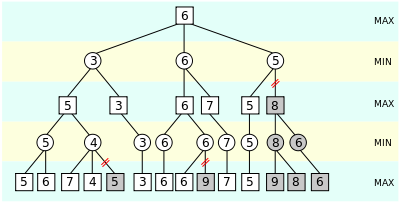
\includegraphics[width=0.6\textwidth]{figures/alpha-beta-pruning.png}
    \caption{Alpha-beta pruning \cite{alpha-beta-pruning}}
    \label{fig:alphaBetaPruning}
\end{figure}

The time complexity of alpha-beta pruning in chess is also dependent on the depth of the search tree and the branching factor of the game. In the worst case scenario, where alpha-beta pruning has no effect, the time complexity is still $O(b^{d})$, the same as for the minimax algorithm. But alpha-beta pruning's time complexity, in the best case, is $O(b^{\frac{d}{2}})$, which is significantly less than that of the classic minimax algorithm.

The effectiveness of alpha-beta pruning depends on the ordering of the moves in the search tree. If the moves are ordered in such a way that the best moves are considered first, then alpha-beta pruning can quickly identify the best move and avoid searching deeper than necessary.

\subsection{Quiescence search}
\label{subsec:ch2sec2subsec3}

When searching for positions, if the search stops after a fixed depth, some of the positions might be in a situation where on the next move the material evaluation could be totally reverted (a big piece about to be captured, a pawn about to be promoted, etc.). In those cases, the evaluation would not be so reliable, and the situation might be reversed in the next move.

To deal with these situations, quiescence search is an improvement that continues the search in non-quiescent positions until a quiescent position is found. A position is considered quiescent if there are no forcing moves (checks, threats) or moves that have a big impact on material (captures, promotions).

% HORIZON EFFECT

\subsection{Iterative deepening}
\label{subsec:ch2sec2subsec4}

When limiting the search by time, performing the minimax to a fixed depth has some disadvantages: if the time has elapsed and the algorithm didn't finish, the results are probably bad, but, on the other hand, if the algorithm finished there might still be some time left, which could be used to improve the result \cite{carolus2006alpha}.

Adrian De Groot, dutch psychologist and chess master, first mentioned the idea of iterative deepening in "Thought and Choice in Chess" \cite{thought2014groot}. With this improvement, the search starts at depth one, and then the depth is incremented and the search is done again, until the given time elapses.

Along with the ability of the algorithm to work well with time limits, iterative deepening introduces an additional advantage: the moves can be ordered at each level using the results given by the previous search, and this has shown to bring improvements to the number of branches cut by alpha-beta pruning.

\subsection{Monte Carlo Tree Search}
\label{subsec:ch2sec2subsec5}

Monte Carlo Tree Search (MCTS) is a search algorithm particularly effective in situations where the state space is large and difficult to exhaustively explore, such as in chess. It is based on the concept of random sampling or simulation. It builds and explores a search tree by repeatedly performing a four-step process:
\begin{itemize}
    \item Selection: starting from the root node of the search tree (the current position), MCTS navigates down the tree by selecting child nodes according to a selection policy, which tipically balances exploration (visiting unexplored moves) and exploitation (favoring moves already visited that have a high win rate)
    \item Expansion: once a leaf node is reached, the algorithm expands the tree by generating other child nodes representing possible moves from that position
    \item Simulation: after expanding the tree, MCTS performs simulations from the newly added child nodes, which involves playing a game from the current state to the end using a simple policy (even random moves) until a terminal state is reached
    \item Backpropagation: the result of the simulation is propagated up the tree, updating the statistics of nodes (for example visit count, win count); this information is used to estimate the evaluation of each node and guide future selection
\end{itemize}

By repeating these steps for a certain number of iterations or until a time limit is reached, MCTS gradually builds up knowledge about the current position.

\section{Evaluation}
\label{sec:ch2sec3}

As mentioned earlier, if unlimited computing power was available, any position could be labeled as winning for white, draw, or winning for black. Because this is not the case, heuristics are used to assign an approximated evaluation to a position.

\subsection{Centipawns}
\label{subsec:ch2sec3subsec1}

The main part of an evaluation function is the material advantage, that is, the number and types of pieces on each side. Pieces are usually assigned a base value, as can be seen in fig. \ref{fig:basicPieceValues}. The king is either assigned no value, because the objective of chess is not to capture the opponent's king, but to checkmate it, therefore its value is considered irrelevant, or is assigned a very high value (bigger than all the other pieces combined), so the engine prioritizes the safety of the king above all else. In this case, the engine would attempt to avoid any moves that might put its own king in danger, even if it means giving up material or positional advantage.

\begin{figure}[h]
    \centering
    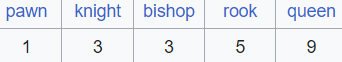
\includegraphics[width=0.4\textwidth]{figures/piece-basic-values.png}
    \caption{Basic piece values \cite{chess-piece-values}}
    \label{fig:basicPieceValues}
\end{figure}

But there are other aspects of a position that need to be taken into consideration by an evaluation function, for example development of the pieces (a piece that is not developed and doesn't attack/defend any squares is not of so much use). Some features of the position are not as important as to add a full point to the evaluation, so usually centipawns are used to evaluate a position. 

For example, some positional advantage a player has might be worth about three quarters of a pawn. A centipawn is a score unit corresponding to a hundredth of a pawn, so three quarters of a pawn would be 75 centipawns. That means a pawn will be worth 100 centipawns, a knight will be worth 300 centipawns, and so on.

\subsection{Handcrafted functions}
\label{subsec:ch2sec3subsec2}

Most engines use a handcrafted function to evaluate positions, measuring features of the board that are considered to give an advantage. Some basic evaluation features are:
\begin{itemize}
    \item Material - the number and types of pieces
    \item Pieces positions - where the pieces are placed (in the center, at the edge, in the corner of the board)
    \item Pawn structure - connected pawns (allied pawns on adjacent files) are considered good, isolated pawns (with no allied pawns on adjacent files) are considered weak, passed pawns (pawns that do not have any opponent pawns on the same file or adjacent files in front of them) are strong, because they cannot be traded by opponent pawns, etc.
    \item Mobility - the number of legal moves a player has in the position
    \item Trapped pieces - pieces that don't have any safe squares to move to are considered weak
    \item King safety - existence of allied pawns in front of the king, distance of opponent pieces to the king, etc.
\end{itemize}

Most of the times, handcrafted evaluation functions also take into consideration the phase of the game - the development of the pieces is the main concern in the opening, followed by attacking and defending in the middle game, and pawn promotion in the endgame.

\subsection{Neural network}
\label{subsec:ch2sec3subsec3}

Another way of building an evaluation function is through training a neural network. Neural networks are a type of machine learning models inspired by the anatomical and functional characteristics of the human brain. They are designed to learn and make predictions or decisions based on input data. Neural networks excel at tasks involving pattern recognition, classification, regression, and other complex data analysis tasks.

Neural networks are composed of interconnected units known as neurons, which are arranged in hierarchical layers including an input layer, one or more hidden layers, and an output layer. Within this architecture, each neuron receives some values as input, applies a mathematical operation, and generates an output that propagates to subsequent layers.

One approach to training the neural network for evaluating chess positions is to use supervised learning, by giving it the position, sometimes along hand-crafted features as input (the ones previously mentioned: material, mobility etc.), and the corresponding evaluations, such as the scores given by human experts or strong chess engines.

Another approach is to use reinforcement learning, where the network is trained by playing against itself and learning from the outcomes of the games. This technique has the advantage of generating its own training data, as well as the ability to find patterns that are stronger and more complex than those that people can think of, if sufficiently trained.